\section{A Refined View of Assurances} \label{sec:synthesis}
    From the review of Quadrants I. through IV. of the formal/informal, explicit/implicit plane, we are able to find some insights with respect to assurances and can discuss them in a more comprehensive way. Using insights from the survey a refined version of Figure~\ref{fig:SimpleTrust_one_way} can be constructed. Figure~\ref{fig:refined_assurances} incorporates all details from Section~\ref{sec:background} as well as adding some insights from the survey. Below we discuss the design of explicit assurances in this more detailed framework (some of these insights might also apply to implicit assurances, but implicit assurances will not be directly discussed in this paper).

    \begin{figure}[htbp]
        \centering
        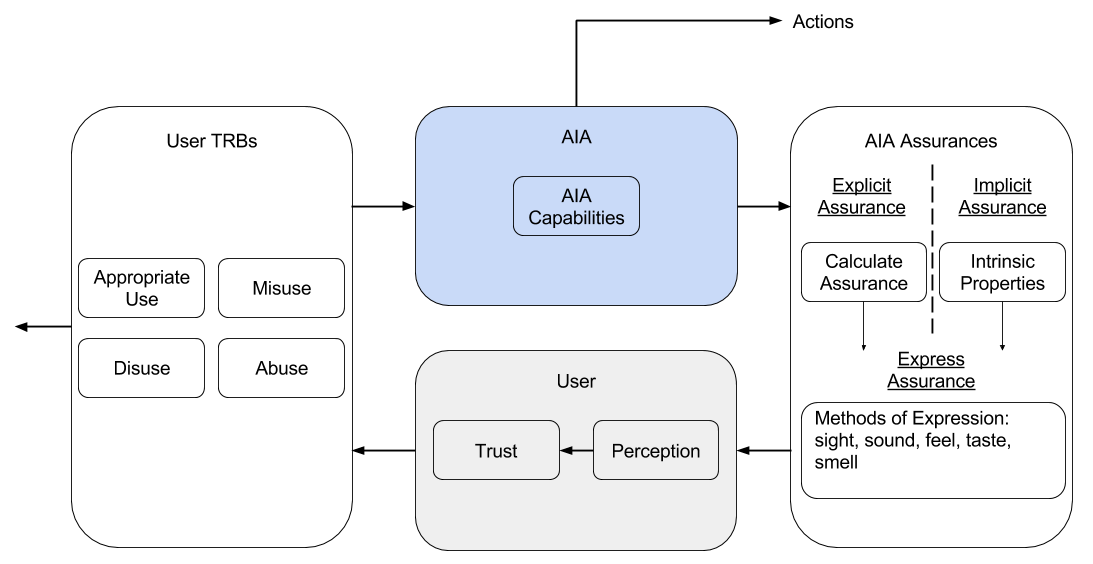
\includegraphics[width=0.9\textwidth]{Figures/RefinedTrust_one_way}
        \caption{Detailed extension of Figure~\ref{fig:SimpleTrust_one_way}. The AIA, User , and User TRBs blocks are defined as discussed in Section~\ref{sec:background} (with the exception of the `Perception' blocks added to the AIA and User boxes). The AIA Assurances box has been filled using insights from the surveyed material. The boxes that are greyed out will not be discussed in this section.}
        \label{fig:refined_assurances}
    \end{figure}

\subsection{Calculating and Planning Explicit Assurances}
    Before giving an explicit assurance to a human user an AIA must first calculate and plan the assurance to be given. There are some explicit assurances that may have been designed into the AIA, that are neither calculated or planned after the AIA has been put into use. One example of an assurance like this might be a static (un-changing) user interface to the AIA. For the purposes of this paper it is more interesting to focus on those assurances that are calculated and planned (although some of the ideas may be useful in designing assurances that are not planned or calculated after deployment of the AIA).

    \subsubsection{Calculating Explicit Assurances}
    From the surveyed material, it seems that there are a few high-level ideas that surround the calculation of assurances, these are: quantifying uncertainty, adding structure, and modifying the AIA objectives.

    \paragraph{Quantifying Uncertainty} Being able to quantify uncertainty in the AIA is a critical step in being able to express that uncertainty to a human user. The general idea is that a model or method needs to be incorporated in the AIA that will represent uncertainty in some way. A human user could use such information to inform their trust in the `situational normality', `competence', and `predictability' of the AIA. We claim that the work surveyed in the sections addressing \nameref{sec:performance_prediction}, \nameref{sec:model_checking}, \nameref{sec:safety}, \nameref{sec:active_learning}, and \nameref{sec:empirical_performance} can be used to this end. Generally these methods are statistical in nature, and directly account for uncertainty.

    This is perhaps the most obvious of the methods to use when attempting to design assurances; In essence trying to provide another layer of information beyond a simple prediction, or recommendation. Generally the surveyed papers from quadrant \ref{sec:q2} found that including things like uncertainty increased the trustworthiness of the AIA in the user's eyes.

    Statistical methods and models are prevalent in the literature surveyed. However, there is still a challenge that exists in creating algorithms that quantify uncertainty for some methods where there is no current, or satisfactory, measure. For example methods that quantify uncertainty in the quality of the solution of a POMDP on an unknown problem, are non-existent or nearly so. This occurrence is not unique to POMDPs, but to many methods that were not designed with uncertainty in mind, this includes things like planners (and plans), optimization algorithms (and the solutions thereof), and learning algorithms (and their predictions).

    \paragraph{Reducing Complexity} Many researchers have attempted to remove complexity from the models and logic of the AIA to make the methods more interpretable to a human user. As with quantifying uncertainty, making an AIA more interpretable can also inform a user's trust in the `situational normality', `competence', and `predictability' of it. Many of the methods applicable were surveyed in the sections regarding \nameref{sec:model_interp}, \nameref{sec:explanation}, \nameref{sec:viz_dr}, \nameref{sec:human_involved},  and \nameref{sec:rep_learning}.

    Generally it is accepted in the surveyed literature that the models and algorithms of AIAs need to have less complexity in order to be better understood by human users. This reduction in complexity was addressed in several different ways, of course the trade-off between model complexity and accuracy is a constant concern. In practice this has been manifest is approaches as simple as making summary statistics, or calculating averages. In more complex approaches several authors (i.e. authors from Section \ref{sec:model_interp} such as \cite{Caruana2015-za}, and \cite{Van_Belle2012-dt}) have attempted to address this issue by using algorithms that are inherently more interpretable while also yielding `world-class' results.

    While it is possible that there are interpretable models that can be designed that can compete with other non-interpretable models, it seems like this may not be the best long-term approach to reducing complexity. We believe that investigating methods that generate explanations from non-interpretable models is a more promising direction. The main reason is that the idea of interpretable models is not well-defined and, in reality, doesn't really exist as a single tangible goal. Instead there is a continuum of interpretability that is based on the complexity of the problem, the time required for a user to interpret (i.e. a few seconds or months of study), the expertise of the user, and others.

    A useful example is explaining one's research to others. When explaining to a researcher from the same field jargon, and shared knowledge can make the explanation easier. However, when trying to explain one's research to a non-expert one must adapt the explanation to be more general and simple; this will inevitably result in the loss of detailed information, but will hopefully convey the main principles to the user.

    To this end, we find work by \cite{Ruping2006-xj}, \cite{Van_Belle2012-dt}, \cite{Ribeiro2016-uc}, and \cite{Choi2016-by} especially interesting. These methods they investigate seem promising in making models have scalable interpretability based on given criteria like required depth of understanding, level of expertise, and time to gain understanding.

    \paragraph{Modified Objectives} The above two approaches alone can largely use existing methods, however some researchers directly modified the methods and models in the AIA to be more meaningful to humans. This was reviewed to some extent in the sections on \nameref{sec:human_involved}, \nameref{sec:active_learning}, \nameref{sec:model_interp} (some researchers modified objectives to learn better models), \nameref{sec:rep_learning}, and \nameref{sec:safety}.

    When \citet{Freitas2006-qo} considered putting a human in the learning process, he essentially modified the objective function of the learning algorithm. In essence the objective function was now based on a large set of human preferences (and biases). This kind of approach is promising, in that it can be used to encode many human qualities that cannot be easily quantified, or even explained. These are trade-offs that can be undesirable in many situations as well. We sometimes use designed objective learning algorithms to avoid human biases. It is interesting that in using a human in the loop can offer more interpretability to a learning process, while at the same time making the learning process itself less procedural. In other words, using a human in the loop can make the result more understandable by a human, but the learning process will be rendered less understandable.

    \citet{Amodei2016-xi} discuss several different considerations related to AI safety, and spend quite a bit of time discussing the situation when AI objectives don't correspond, or align, with human objectives (this is something addressed in a specific situation by \cite{Hadfield-Menell2016-ws}, also \cite{Bostrom2012-uf}). One of the main insights is that the source of discord between what humans expect and what AIAs actually do is because of poorly designed objective functions that you might refer to as myopic, or focusing on a specific objective to the extent that a human can no longer relate to the objective of the AIA. This suggests to designers that significant time may be required to design objectives that align with human objectives, this alignment will automatically make the AIA more predictable, and competent in the user's eyes.

    \subsubsection{Planning Explicit Assurances}
    Planning assurances is critical when trying to attain desired TRBs from a human user. However, planning is not available to all levels of AIA complexity. In cases where AIAs don't have the ability to plan during usage, they may be designed beforehand with some kind of static plan of assurance. Otherwise, in more advanced AIAs, the AIA might take into account TRBs to plan an assurance strategy to assist the human to use it appropriately.

    When planning assurances the AIA must be able to account for limitations of users, and its own limitations in expressing assurances. For example a user may not be able to understand the necessary information needed to use the AIA more appropriately. Also, the AIA may need to take a long-term strategy to teach the user, as opposed to only presenting the user with canned, static, assurances. Some of the important user considerations will be discussed further in Section~\ref{sec:express_assurances}.
    
    \paragraph{User Cognition:} Part of the consideration for planning an assurance is whether the human user can correctly process the information received. This is perhaps most easily illustrated by considering a non-expert user who cannot understand highly technical assurances regarding the AIA. However, less trivial manifestations may be troubling. This point was not directly addressed in the survey papers, but evidence of its existence were seen. For example \cite{Riley1996-qm}, and \cite{Freedy2007-sg} both observed evidence of framing effects (the tendency of a user to become too trusting once they are in the mode of trusting). This suggests the existence of other kinds of typical cognitive behaviors such as recency effects (having biased trust based on recent experiences), and the existence of bias in the perception of assurances.

\subsection{Expression and Perception of Assurances} \label{sec:express_assurances}
    Expression and Perception of assurances have been combined in this section because they share several critical aspects. In designing assurances the medium, and method of expression must be selected taking into consideration the limitations of the AIA. Here medium denotes the means by which an assurances is expressed, this could be through any of senses by which humans perceive, such as sight, sound, touch, smell, and taste. The method of assurance is the way by which the assurance is expressed. An example may help: a plot may be conveyed through sight in the typical way, or through words (for example when communicating to a blind person); in this case the plot is the method, and sight or sound are the different mediums through which it can be communicated. An AIA might be limited in expression because it does not have a display, or a speaker.

    A designer must also consider whether a human can perceive the assurances being given. If so, to what extent is the information from the assurance transfered (i.e. how much information was lost in the communication)? A few examples include: an AIA giving an auditory assurance in a noisy room and the user not hearing it (such as an alert bell in a factory where the workers use ear-plugs), or an AIA attempting to display an assurance to a user that has obstructed vision.
    
    If an assurance is not expressed, or not perceived by the user, it is useless and has no effect. For example, an AIA may have the ability to store data about its performance, and compute a statistic regarding its reliability, but if it cannot express (or communicate) that information in some way, the information is useless.

    A user will always have some kind of TRB towards an AIA (if only to choose to ignore the AIA). In the absence of explicit assurances the human will instead use implicit assurances to inform their TRBs. However, the general human user will not have knowledge regarding which assurances are implicit or explicit (humans participating in research from Quadrants I and II were not aware which assurances were implicit or explicit). In other words the user won't necessarily be able to distinguish which assurances were designed and which weren't. To the user all assurances are the same, that is to say that any property or behavior of an AIA that affects trust is an assurance, and it doesn't matter whether the assurance was designed or not (is explicit or implicit).
    
    The expression and perception of assurances to a human user is not a trivial topic and has been investigated mainly by those in Quadrants I, and II  when utilizing basic visualizations and natural language communication (some other promising approaches like high dimensional visualization were mentioned in Quadrants III and IV). There is, however, a body of research (not surveyed here) that considers methods by which to communicate information to humans (i.e. as probabilities, or fractions, by text, or by plotting, etcetera). It is probable that the fields of marketing, and cognitive science have much to contribute to this topic. This research is critical in designing how to efficiently express assurances in a way that they will be perceived correctly by the user with the least possible information loss.

    \paragraph{Methods:} As already mentioned, approaches such as showing plots, displaying natural language, visually projecting plans, and displaying summary statistics, have been investigated in the surveyed literature. Their effect has been observed in some instances by use of TRBs and self-reports from users. However, it is generally unclear how appropriate these methods are, and in which situations they should be used, and so there remains much research to be done in this area.

    Perhaps more importantly there are several potential sources of explicit assurance that lack appropriate expressions, and thus cannot be effectively utilized as assurances. For example, it is unclear the best way for an AIA to express that it has been validated and verified on situations similar to the current one. Similarly, what other methods exist for communicating statistical distributions besides showing a plot (only useful for 1 or 2 dimensional distributions) or showing sufficient statistics? Investigating how assurances can be expressed in effective, and efficient ways is critical to human-AIA trust relationships.

    \paragraph{Mediums:} In this survey we saw several different mediums used to convey an assurance. Some used sight such as in \cite{Chadalavada2015-wx} where the robot gave visual feedback to a user, or in \cite{Muir1996-gt} where performance data were visible on a computer screen. Others used sight as well when communicating via natural language (i.e. \cite{Wang2016-id}) -- it is also a simple matter to convert natural language output from visual to auditory with existing technology. Generally, any human sense could be used as a medium, besides sight, and sound this includes touch, smell, and taste. None of the last three have formally been investigated in human-AIA trust relationships to our knowledge. Although it should be said that haptic feedback (where the user receives mechanical feedback through the robot controls) is frequently used as a part of a more immersive user interface in robotics. Taste and smell have an obvious application in the assurances of a cooking robot.

    \paragraph{Efficiency:} Some kinds of expression are very `one-dimensional' in that they only use one medium, or method. This, again, is seen in practice by utilization of plotting a certain value over time. Because of this much of the research to date involves assurances that are not robust to loss in transfer. Because of this, exploring ways in which assurances can be robustly communicated is a clear opportunity for those trying to design assurances. This is akin to a human speaking with their voice, making facial expressions, and gestures with their hands as well; simultaneously utilizing several mediums/methods helps to ensure an assurance will be perceived correctly. Of course, repeating the same message over a thousand times is wasteful, and so enters the idea of efficiency in expression.

    Perhaps less obvious is a situation in which the user has to supplement an incomplete assurance. As a simple example, in \cite{Muir1994-ow} a simple flow-rate is provided to the user, they then supposedly create a mental model of the reliability -- based on repeated observations over time of the AIA to inform their TRBs. Creating this mental model takes time, and the model is prone to cognitive biases (discussed a bit more below). In this case the assurance is communicated slowly and indirectly.
    
    Generally, a highly efficient assurance would have precise information communicated in a way that is easy for the user to perceive, with little loss. Whereas, an inefficient assurance may be more vague, wasteful (i.e. repeating the same thing a thousand times), and susceptible to loss in communication. The likely solutions to efficiency lay in selecting appropriate methods, and mediums for expression of the assurance.

    \paragraph{Implicit and Explicit Assurances:} It is worth considering, in more detail, what implications this has on the designer. The foremost consideration is that an analysis of the interaction between the human and user need to be made in order to identify the critical assurances for a given scenario. For example, in the road network problem, an analysis might find that the most critical assurances are about the competence of the UGV's planner. In this case the designer must take time to design a planning-competence assurance.

    One difficulty arises form this approach, which is that there doesn't seem to be a way to determine what passive assurances might drown out active assurances. Following from the example above, the designer may have built an excellent planning-competence assurance, but failed to consider the effect of how the UGV appears -- it may be old, have loose panels, and rust holes. Generally, designers overlook implicit assurances (i.e. do not consider them explicitly in design) because they assume that they will have no effect (i.e. why does it matter if there are rust-holes if the UGV works?). This can stem from either: 1) ignorance of human-AIA trust dynamics, or 2) lack of identifying which assurances are most important to a human user.

    While it might be nice, it seems unreasonable, inefficient, and unwise to perform a study of \emph{every possible} assurance from an AIA to a human and then select the most important. Perhaps one way a designer might try to identify which assurances are important is to perform human studies where feedback about which characteristics of the AIA most affected the trust of the user. An approach like this would help to point out if explicit assurances are being noticed, and if there are implicit assurances that are overly influential, or that overwhelm the explicitly designed assurances. With such feedback designers would have a realistic idea about whether their explicit assurances are having the desired effect.

    \paragraph{Human-like assurance:} It is generally presumed that making something more human-like will make an AIA more trustworthy. An algorithm may be human-like when it represents knowledge in a way that a human would understand, or executes logic in a way that a human can follow. A robot that is humanoid becomes more human-like in appearance (as investigated in \cite{Bainbridge2011-pl}), a system that uses natural language becomes more human-like in communication (for example in \cite{Lacave2002-cu}). Generally, since human-AIA trust relies on an interface between humans and AIAs, there must be some kind of method by which the AIA and human draw closer together in some way. As humans are the designers of AIAs this is typically done by making an interface where the AIA become more human-like, by implicit or explicit means, if only when it comes time to express assurances.

    Contrasting \cite{Dragan2013-wd} and \cite{Wu2016-ei} shows that sometimes the same technique can have different effects when used in different situations. In \cite{Dragan2013-wd} the AIA is made more trustworthy by making the robot motions more human-like, whereas in \cite{Wu2016-ei} making the AIA more human-like resulted in a decrease of trustworthiness. In this case the difference came from the type of task, in the first case the robot was physically working in proximity to a human, in the other case the user was playing a competitive game against the AIA.

    We therefore see that making a system more `human-like' can both positively and negatively affect trust between human and AIA. 
    \citet{Tripp2011-rx} noted that humans trust more `human-like' AIAs in more human-like ways. Perhaps in this case `human-like' applies to how difficult it is to fully understand and predict the AIA. This is definitely true with humans, one can never be sure how a human will act in given situations. Following on this idea the benefits or drawbacks of human-like characteristics are likely amplified by the risk of the situation in which being unpredictable is not conducive to increased trust.

\subsection{Measuring the effects of Assurances} \label{sec:measuring_effects}

    There are two different situations when it would be desirable to measure the effects of assurances. The first is when the designer wants to understand the effectiveness, the second would be when the AIA itself needs to measure whether assurances are effective or not. To our knowledge there has not been any work regarding the second situation where an AIA would measure response to assurances and then adapt behaviors appropriately (at least not in the trust cycle setting), however this is arguably the ultimate goal so that AIAs can themselves modify assurances to meet different needs. What does this mean practically? It seems that any method that is made for the designer to measure the effects of assurances could also be deployed into an AIA. The surveyed literature gives some insights into how that has been done to date.
   
    When it comes time to measure the effect of assurances on a human's trust there are two main approaches. The first is self-reported changes based on questionnaires, the second involves measuring changes of user's TRBs. The questionnaire approach was used extensively in many of the papers surveyed, questions like `how trustworthy do you feel the system is?', or `to what extent do you find the system to be interpretable?'. These kinds of questions can be useful in verifying whether the assurances are having the expected effect. It is not unreasonable to imagine that an AIA might be equipped with a method by which it can ask the user questions about their trust, process those responses, and modify assurances appropriately.
    
    However, evidence is presented in \cite{Dzindolet2003-ts} that illustrates that sometimes changes is self-reported trust do not result in changes in TRBs. From the AIAs perspective this means that --- unless the object of the assurances is to make the person's level of self-reported trust change --- the assurances are not providing any benefit. As previously discussed, the goal of assurances is to elicit appropriate TRBs from the human user. From this perspective, measuring changes in TRBs is the more objective approach to measure the effect of assurances.

    Generally researchers in the field have measured, in some way, how frequently the AIA was able to run in autonomous mode, before being turned off. This metric seems very reasonable, and seems to be a promising approach with some extensions. Perhaps a better defined metric would be the likelihood of appropriate use of a certain capability by the user. For example in the UGV road-network example there isn't really an option to `turn off' the UGV. Instead the remote operator can make decisions such as accepting a plan designed by the UGV. In this situation the effect of assurances might be measured by how likely the operator is to accept a generated plan instead of overriding it (recall that the goal may not be to have the generated plan accepted 100\% of the time, rather that it be accepted with respect to how appropriate it is in a given situation).

    Self-reports are likely the most useful when trying to understand the true effects of an assurance. Does a certain assurance, assumed to affect `situational normality', actually do that? There is space for quite a lot of research in this realm. Does displaying a specific plot actually convey  information about `predictability'? This information can be used to inform the selection of the methods of assurance.

    In practical application (such as in the UGV road-network problem), the user, and the human-AIA team, care more about whether TRBs are appropriate or not. It doesn't help if an assurance helps the user feel that the AIA is more competent, if the user doesn't treat the AIA any differently than before the assurance. This assumes that it is possible for appropriate TRBs be measured in the first place. For example, if appropriate behavior is for the user to verify a sensor reading, can the AIA perceive that? In that situation perhaps the easiest approach would be to ask the user, but what if the user lied? Is there a way to verify the TRB is actually appropriate? This is something that has gained notoriety with autonomous cars, where the car can drive itself, but the user still needs to sit in the driver's seat and be attentive just in case the vehicle cannot perform correctly. We claim that it is as important to design methods of perceiving appropriate (and inappropriate) TRBs as it is to design assurances. 
%
% \subsection{The Imprecise Nature of Assurances} \label{sec:imprecise_nature}
    % Due to the nature of trust (and humans in general), a single assurance might be targeted at influencing the competence dimension of trust, but it may also have effects on other dimensions. As an example an assurance that targets predictability may also have an affect on the probability of depending.
%
    % Besides being difficult to separate effects on a single user, individual users are different as well. Thus no assurance will have an identical effect when given to two separate users. This makes it difficult to have precise effects on user trust behaviors.
%
    % One might attempt to mitigate this uncertainty by using expressions that are more precise than others, such as displaying a probability distribution rather than on a maximum likelihood. This gets into some considerations about how the presentation of information affects the ability of a human to understand.
